\chapter{Introduction}
\label{chap:introduction}
% -----------------------------------------------------------------------------

This is the report of a semester project (PS6) done at the \acrfull{heia} in collaboration with the company \acrfull{dec}.
The goal is to achieve a connected dispenser that allows micro-dosing of liquid for drug production.

Today, drug production faces many challenges, she is becoming more and more complex and the demand is increasing.
We have seen during COVID-19 that the industry has had difficulties in meeting the demand.
To avoid this happening again, it's important to find solutions to increase production agility.
Currently, the production of drugs is done in huge quantities and the goal of this project is to provide a solution for small batch production and laboratory testing.

\acrfull{dec} is a Swiss-based multinational company that is specialized in pharmaceutical, chemical and cosmetic production equipment for over 35 years.
This company is at the origin of the creation of the $\mu$BoMa which is a microdispenser that answers the demand for small batch production.

The goal of this project is to realize the connected part of the $\mu$BoMa.
We want to be able to use the microdispenser in a production line that can manage up to three dispensers at the same time and in a laboratory environment where a smartphone or other personal device can control the dosage.
For this, it will be equipped with a microcontroller that will have a module to network with other devices.
We can imagine wifi and Bluetooth but it remains to be defined.


\section{Goals}
\label{ch:introduction:goals}

This project has two main goals, the first one is to control the microdispenser and the second one is to provide an interface to manage it.
The first goal is the most important because it's the blocking point of the project.
The second goal is the one that will be the most visible to the user.
The goal is to provide an interface that can be used in a production line and in a laboratory environment.
The laboratory environment will be prioritized but it's important to keep in mind that the production line will be the final goal and this service must be over ethernet and the protocol \acrfull{opc}~\cite{opc}.

There are also optional goals that will be done if the time allows it.
These goals are the implementation of the standard SiLA and \acrfull{mtp}.
There are standards that are used in the pharmaceutical industry and it could be interesting to implement them to make the integration much easier.
There is also the development of multiple interfaces like a REST API or the Bluetooth.

At the end of the project, the \acrshort{mvp} will be able to control and read the information of the microdispenser.
It will also provide an interface to manage it.
The code is destined to be changed and improved in the future, so it will be written in a way that it can be easily modified.


\section{Planning}
\label{ch:introduction:planning}

The activities of the project will be separated in two parts.
The first one will follow a sequential model until the blocking points are done.
The second one will be a methodology by iteration to complete the milestone about the application interface and the next.
The method will change because the number of features isn't known yet and the needs can change.
The following figure \ref{fig:planning} shows the different steps of the project and how the milestone will be achieved.

\begin{figure}[ht]
    \centering
    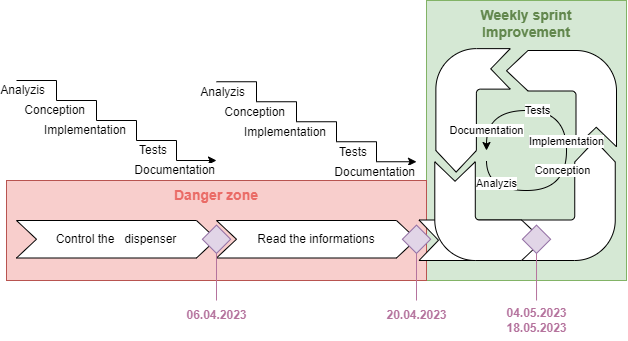
\includegraphics[width=1\textwidth]{img/planning.drawio.png}
    \caption{Planning}
    \label{fig:planning}
\end{figure}

The danger zone is the part of the project where the blocking points are.
It represents by the red part of the figure \ref{fig:planning} these steps are required to go further in the project.

The agile part represents the task that will be done to improve the project.
That's in this part that the client application will be done and the optional goals will be implemented.
